% Chapter 3

\chapter{Methodology and Tools} % Write in your own chapter title
\label{Chapter3}
\lhead{} % Write in your own chapter title to set the page header

\section{Pipeline 1 - ConvMC-Net}
\subsection{General Methodology}
% We reverted to convolution maps as that has been shown to perform amazingly well in deep unfolded approaches (maybe cite some resouces like ISTA being unfolded etc) So now borrow content from shoaib bhai paper of ConvMC and mention the classic augmented lagrangian approach + CNNs to give rise to ConvMC net. Mention how it was trained (from synthetic generation - explain breifly i.e. the vanilla problem with simple white noise so far). Can even show the architecture diagram as well here. 
Now that we have discussed in quite detail the various algorithms and optimization techniques for matrix completion problem and the essence of model-based deep learning, we propose \textit{ConvMC-Net} our first model combining the systematic connections built in the already fine-tuned optimization algorithm namely ADMM (discussed in previous chapter) and unprecedented performance gains we aim to gain from the inclusion of deep learning methods. 

As the name suggests, ConvMC-Net uses learnable convolution kernels, which are learned from data, in its unfolding process. We trained our model on two tasks, i) Synthetic Dataset and ii) Image Inpainting. We utilized the unfolding of a \textit{vanilla} formulation with no noise component in our objective function. This was done mainly to test how much one can trust the 'learning' paradigm even when it will be faced with 'seemingly' out of distribution problems i.e. matrix recovery in the presence of noisy entries. More details later in section 3.1.3.

The synthetic dataset ground labels were constructed from a product of two normal distributed matrices and then a mask of same shape as the product with entries of 1/0 randomly chosen was multiplied to give the low-rank matrix. We varied the level of white noise (variance) and the sampling rate to get various datasets. Further, seeing that matrix completion problems are prevalent in wireless sensor networks, we also trained the model on a on a real-world sensing dataset. It consists of temperature data collected every 30 seconds by 54 sensors distributed in Intel Berkeley Research Lab \cite{intelberkeley2004}. Further, for image inpainting we resorted to using the CSDS 300 Color dataset \cite{MartinFTM01} consisting of 200 train images and 100 test image.. The training process used the original matrices as the ground truth and low-rank as the input. Finally, as discussed in detail later in section 3.1.3, we transitioned from a simple white noise to GMM noise, a problem that is recently being dealt when it comes to robust matrix completion for e.g \cite{lo-bcd}. This is not the end for our dataset creation methods as during our experimentation, we found several algorithms performing better/worse if the matrix dimensions were to increase/decrease. Hence we resorted to the above datasets in two formats i) $150 \times 300$ and ii) $400 \times 500$. 

For comparison purposes we resorted to first dealing with a similar deep unfolding approach (mentioned before) of ADMM-Net. Our experiments on a real world dataset of a sensor network show that the proposed ConvMC-Net is significantly faster than ADMM-Net in both training and at inference while giving better accuracy and showing improved robustness. Moreover, the number of layers of ConvMC-Net can be increased very easily for improved convergence, if needed, and it is also easily applicable on high dimensional matrices. Therefore, we later switched to comparing with other several prominent algorithms. 

\subsection{Data Selection}

For a problem as matrix completion or any other low rank approximation or matrix factorization or mostly any problem that can be formulated as a matrix recovery problem through regression or other such frameworks, synthetic datasets provide an amazing flexibility. Not only it is simple, straightforward but we can theoretically generate as many samples we want. For this reason, as well as other prominent methods, they always test their performance on synthetic datasets before going for challenging their models in real-life scenarios such as image inpainting or hyperspectral imaging. The synthetic dataset generation for GMM noise is explained below. Note the case for simple white gaussian noise was similar except the pdf of the noise changed from a GMM pdf to simple normal distribution. 

The noise-free and complete matrix $X \in \mathbb{R}^{400 \times 500}$ with $r = 10$ is generated by the product of $X_1 \in \mathbb{R}^{400 \times 10}$ and $X_2 \in \mathbb{R}^{10 \times 500}$ whose entries obey the standard Gaussian distribution. Then, the incomplete matrix without noise $X_{\text{incomplete}}$ consists of randomly selected 50\% entries from $X$. In other words, 50\% entries of $X_{\text{incomplete}}$ are equal to 1, and the rest are 0. Moreover, $X_{\text{incomplete}}$ is added with independent impulsive noise which is modeled by Gaussian mixture model (GMM). The probability density function (PDF) of GMM is given by
\[
p_v(v) = \frac{c_1 }{\sqrt{2\pi\sigma_1^2}} \exp\left(-\frac{v^2}{2\sigma_1^2}\right) + \frac{c_2}{ \sqrt{2\pi\sigma_2^2}}\exp\left(-\frac{v^2}{2\sigma_2^2}\right)
\]
where $c_1 + c_2 = 1$ with $0 < c_i < 1$, and $\sigma_1^2$ and $\sigma_2^2$ are variances. To simulate the impulsive noise, it requires $\sigma_2^2 \gg \sigma_1^2$ and $c_2 < c_1$. It means that sparse and high power noise samples with $\sigma_2^2$ and $c_2$ are mixed in Gaussian background noise with small variance $\sigma_1^2$. In our simulations, we set $\sigma_2^2 = 100\sigma_1^2$ and $c_2 = 0.1$. The signal-to-noise ratio (SNR) is defined as
\[
\text{SNR} = \frac{\|X_{\text{incomplete}}\|_F^2}{\sigma_v^2}
\]
where $\sigma_v^2 = \sum_{i=1}^{2} c_i \sigma_i^2$ is the total noise variance.

The recovery performance is measured by mean squared error (MSE), defined as
\[
\text{MSE} = \frac{\|M - X\|_F^2}{mn}
\]
where $M$ is the recovered matrix.

We followed a similar process for the image inpainting dataset CSDS 300 which consisted of 200 train images and 100 test images. Each image was RGB format and 481 x 321 hence was appropriately gray-scaled, resized before passing it to the data generation above. 

As for the preperation of the real-world sensing dataset, its laid down in Chapter 4. 

\subsection{Deep Learning Architecture and Final Design}

% Explain in detail the the architecture starting from the problem formulation toaugmented lagrangian to ALM algorithm to CNN utilization (basically shoaib paper stuff). But in this section in detail explain the slump we faced here when comparing results on image inpainting/synthetic datasets with the GOAT L0-BCD (vanilla problem vs GMM noise problem) which eventually led us to M-estimation. But also mention we later tried it on GMM corrupted data as well (synthetic + image inpainting both but very sus results i.e. same trajectories of loss)
In this section, we go through the technical details of our model ConvMC-Net and its first competitor ADMM-Net. We start of with the formulation of ConvMC-Net derived from the vanilla problem structure solved through \textit{augmented Lagrange multiplier} method. 

MC aims at restoring the original matrix $D_{M \times N}$ from its undersampled/incomplete version $D_{\Omega}$, expressed as
\[ D_{\Omega} = U \odot D, \]
where $\Omega$ is a subset containing 2D coordinates of sampled entries, $\odot$ represents the Hadamard product, and $U$ represents the sampling matrix. Furthermore, it is assumed that $D$ is low-rank. NNM setup is the following:
\[
\min_L \|L\|_*, \text{ such that } D_{\Omega} = L_{\Omega},
\]
where $\|.\|_*$ represents the nuclear norm of a matrix defined as the sum of the singular values of $L$, and $L_{\Omega}$ denotes the projection on $\Omega$. We formulate above in an augmented Lagrangian form as
\begin{equation}
    L(L, Y) = \|L\|_* + \text{Tr}(Y^T \cdot (D_{\Omega} - L_{\Omega})) + \frac{\mu}{2} \|D_{\Omega} - L_{\Omega}\|_F^2,
\label{eq: 22}
\end{equation}

where $\|.\|_F$ denotes the Frobenius norm, $\text{Tr}()$ denotes the trace of a matrix, $Y$ is the Lagrange multiplier of size $M \times N$, and $\mu$ is a regularization parameter that controls the penalty for violation of linear constraints. The augmented Lagrangian method seeks a saddle point of $L$ by alternating between minimizing with respect to the primal variable $L$ and taking one step of gradient ascent to increase $L$ using dual variable $Y$ as
\begin{equation}
    L^{k+1} \in \min_L \frac{1}{\mu} \|L\|_* + \frac{1}{2}  \|D_{\Omega} - L_{\Omega} + \frac{Y}{\mu}\|_F^2,
    \label{eq: 17}
\end{equation}

\[ 
Y^{k+1} = Y^k + \mu \nabla_Y L(L^{k+1}, Y^k),
\]
where $\nabla_Y L(L^{k+1}, Y^k)$ denotes the gradient of \ref{eq: 22} with respect to $Y$. We then solve \ref{eq: 17} using ISTA, the iterative step of which is given as
\begin{equation}
    L^{k+1} = \text{prox} \left( L^k - \frac{1}{\mu} \nabla_L L^k \right),
    \label{eq: 18}
\end{equation}

where $\text{prox} (.)$ denotes the proximal operator and $\nabla(L)$ denotes the gradient of the quadratic part with respect to $L$. The proximal operator for computing the low-rank component is the singular value thresholding operation, $\Psi_{\alpha}(X) = U \text{diag}(\text{Relu}(\sigma_i - \alpha))V^H$, where $X$ has an SVD given by $X = U\Sigma V^T$, $\text{diag}(y_i)$ represents a diagonal matrix with its $i^{th}$ diagonal entry equal to $y_i$, and $\sigma_i$ represents the $i^{th}$ singular value of $X$. The resulting procedure is stated in Algorithm 5. 

\begin{algorithm}
\caption{Matrix Completion by ALM}
\begin{algorithmic}[1]
\State \textbf{Input:} Initialize: $L^0 = Y^0 = 0$, $\mu > 0$
\State \textbf{Output:} $L$
\While {not converged}
    \State $L^{k+1} = \Psi_{\mu^{-1}} \left\{ L_{\Omega^C} + D_{\Omega} + \mu^{-1}Y_{\Omega} \right\}$, where $\Omega^C$ denotes the complement of set $\Omega$
    \State $Y^{k+1} = Y^k + \mu(D_{\Omega} - L^{k+1}_{\Omega})$
\EndWhile
\State \textbf{Return} $L$
\end{algorithmic}
\label{algo: 2}
\end{algorithm}

Although there are different ways \cite{way1, way2, way3} to unfold an iterative algorithm into a DNN, we follow the method of \cite{way1} in unfolding Algorithm \ref{algo: 2}. Hence, we introduce a measurement matrix $H$ into \eqref{eq: 17} as follows:
\begin{equation}
\min_L \frac{1}{\mu} \|L\|_* + \frac{1}{2} \|D_{\Omega} - (HL)_{\Omega} + \frac{Y_{\Omega}}{\mu}\|_F^2 \label{eq: 19}
\end{equation}
We further replace $(HL)_{\Omega}$ with $GL_{\Omega}$ on the basis that there exists a matrix $G$, corresponding to $H$, such that $\|(HL)_{\Omega} - GL_{\Omega}\|_F < \epsilon$. Using \ref{eq: 18}, the iterative step for $L$, after some algebraic manipulation, turns out to be:
\begin{equation}
\begin{aligned}
L^{k+1} = &\Psi_{\frac{1}{\mu^k}} \{L^{k} + G^T D_{\Omega} - G^T G L^{k}_{\Omega} + \frac{G^T}{\mu^{k}} Y^{k}_{\Omega} \}
\end{aligned}
\label{eq: 20}
\end{equation}
We unroll \ref{eq: 20} into the multi-layer neural network of ConvMC-Net by replacing the functions of the matrix $G$ with learnable parameters. Consequently, we replace $G^T$ and $G^T G$, multiplied with $D_{\Omega}$ and $L^{k}_{\Omega}$, respectively with convolution kernels.

In case of the Lagrange multiplier $Y$, we consider for a fixed $G$, two matrices $W$ and $B$ such that $G^T Y_{\Omega} = W \circ Y_{\Omega} + B$.

Finally, we write the deep unfolded version of \ref{eq: 20} as:
\begin{equation}
L^{k+1} = \Psi_{\frac{1}{\mu^{k}}} \{L^{k} + (C^{k}_{1} * D) + (C^{k}_{2} * L^{k}_{\Omega}) + (W_k \circ Y^{k}_{\Omega} + B^k)\}
\label{eq: 21}
\end{equation}
where $*$ denotes the convolution operation, $C^{k}_{1}$, $C^{k}_{2}$ are the convolution kernels learned in the $k$th layer of ConvMC-Net together with the matrices $W^k$ and $B^k$ and the regularization parameter $1/(\mu^k)$. Experimentation details such as epochs, etc are mentioned in chapter 4. We move on with the formulation of ADMM-Net. 

ADMM-Net is derived from unfolding the iterative steps for solving the following minimization problem:
\begin{equation}
\begin{aligned}
\min_{L,Z} & \rho \|Z\|_* + \frac{1}{2} \|D_{\Omega} - L_{\Omega}\|_F^2 + \frac{\lambda_1}{2} \|L^T\|_F^2 + \frac{\lambda_2}{2} \|SL\|_F^2, \\
& \text{such that } L = Z, \label{eq:admm-net-problem}
\end{aligned}
\end{equation}
where $\lambda_1$, $\lambda_2$, and $\rho$ denote the regularization parameters, $Z$ is a slack variable, $T$ represents a differential operator \cite{mao2018spatio} such that $LT = [l_2 - l_1, l_3 - l_2, ..., l_N - l_{N-1}]$, and $S$ represents the spatial relation among measurements of different sensors \cite{mao2018spatio} such that $SL$ gives the spatial difference of $L$. Minimizing $\|LT\|_F^2$ enforces temporal consistency of the sensor readings whereas minimizing $\|SL\|_F^2$ enforces spatial correlation between sensor readings. The deep unfolded steps of ADMM-Net are then written as
\begin{align}
\text{vec}(L^{k+1}) &= (\tilde{U} + \lambda^k_1\tilde{T} + \lambda^k_2\tilde{S} + \zeta^k\tilde{I})^{-1} \text{vec}(\zeta^k(Z^k - P^k)) + D_{\Omega}, \label{eq:admm-net-step1} \\
Z^{k+1} &= \Psi_{\tau^k} \left( L^{k+1} + P^k \right), \label{eq:admm-net-step2} \\
P^{k+1} &= P^k + \eta^k (L^{k+1} - Z^{k+1}), \label{eq:admm-net-step3}
\end{align}
where $\zeta$ is a penalty parameter introduced when making the augmented Lagrangian from \ref{eq:admm-net-problem}, $\tilde{I}$ is the $MN$ dimensional identity matrix, $P = M/\zeta$ where $M$ is the Lagrange multiplier, and $\tilde{U} = \text{diag}(\text{vec}(U))$. Furthermore, $\tilde{S} = I_N \otimes ((S_k)^T S_k)$ and $\tilde{T} = (T^T T) \otimes {I_M}$, where $\otimes$ represents the Kronecker product. The parameters $\{S^k, \lambda^k_1, \lambda^k_2, \zeta^k, \tau^k, \eta^k\}_{k=1}^K$ are learned by the network at every layer in ADMM-Net.

\section{Pipeline 2 - Huber Approach}
% Exact same subsections as above pipelines 
\subsection{General Methodology}
As already discussed much in chapter 2 about the approach of matrix factorization to solve matrix completion, we transitioned from the above ADMM to such an approach. This was done due to few reasons and had several benefits. The objective function above dealt with in both ADMM-Net and ConvMC-Net is a non-smooth convex optimization problem because of the presence of the nuclear norm. Moreover, due to such non-smooth techniques, techniques like ALM/ADMM are required which are further equipped with 'proximal' step updates to deal with the non-smooth term. This as we have seen above, requires the use of SVT. And since our main aim from the start was to improve accuracy but also as importantly as inference, we resorted to convex-optimization problem formulations that do not require such SVD calculations especially at each iteration of the algorithm. Moreover, as far as we have seen very few if not none have attempted at unfolding such smooth convex-optimization problems. One might infer it might be that DNNs love non-smooth updates like that of proximal updates and optimal updates found in convex problems are not so beneficial for DNNs to bank on. Again this was a hypothesis at the start and only through experimentation could we validate this claim. 

The last reason why we tried unfolding matrix factorization approaches is because the classic ADMM approach as seen in ConvMC-Net did not even have a sprinkle of noise assumed in its objective formulation. This is because as shown above that such methods are not equipped to deal with complex noise distributions especially GMM which is at the center of research right now. However, note that variants of such Principal Component Pursuit (PCP) methods do exist such as Accelerated Proximal Gradient \cite{apg} but that adds increased complexity. That can be a another research attempt for another time however, matrix factorization are flexible enough to deal with such complex noise distributions and do not require expensive computation like SVD. Therefore, this is why we tried to go ahead with the unfolding of such algorithms hoping for further improved inference and accuracy,

In general the methodology we adopt to unfold here unlike ConvMC-Net before with the inclusion of CNN's, we go ahead with one of the most prominent algorithm in fields of signal processing i.e. majorization-minimzation (MM) approach \cite{lange_mm_algorithm} based algorithm known as 'Huber' Regression. It employs one of the famous 'Huber Criterion' \cite{huber_criterion} as its smooth convex optimization problem effectively updating the matrix factors as sub-regression problems. More details regarding this algorithm, its unfolded version, its strong competitors \(\ell_0\)-BCD and \(\ell_p\)-reg will be discussed in much technical detail.

% start of by saying since we were comparing results with one of the top state of the art methods L0-BCD, we found it best to use of its tough competitiors through an unfolding approach. We came across M-Estimation techinque and Huber's Criterion a convex optimization problem with little to no computationally heavy operations like SVD. We utilized the MM algorithm in its iterative version (maybe link the Original huberreg - later proved to be wrong) by treating the matrix factorization as a simple regression problem. Training same as before but not on simple white noise data anymore but GMM corrupted data. 
\subsection{Data Selection}
We ignore this section for this pipeline as we follow the exact pipeline mentioned above in section 3.1.2. The details of the training process can be found in chapter 4. 
\subsection{Deep Learning Architecture}
% Explain in detail the algo (add it) and the architecutre (add pic if possible) of the original hubermc and its performance (again along the lines of fluctuation etc i.e. borrow content from section 4 of compilation). We then moved on the real hubereg found from our studies of Robust Signal Processing book etc mention the algorithm here followed by its unfolded architecture (with its cnns added) and its performance. Remember to include our tries of even learning X+. (failure performance - same performance throughout) 

We first discuss and motivate why one should adopt the MM method and Huber's criterion for a classical regression problem. Consider the following. 

Often the regression model also includes a constant term and, for this case, the model is
\[
y_i = \beta_0 + x_{[i]}^T\beta + v_i, \quad i = 1, \ldots ,N,
\]
where $\beta_0 \in \mathbb{F}$ is called the intercept. The model can be written in the form (2.7) by letting $x_{i} = (1, x_{i1}, \ldots , x_{ip})$, $i = 1, \ldots ,N$, be the vector of predictors for the $i$th response and $\beta = (\beta_0, \beta_1, \ldots , \beta_p)$ be the regression vector. When the vector notation of (2.8) is used, $X$ has size $N \times (p + 1)$, the first column being the $N$-vector of ones, denoted by $\mathbf{1}$. In this case, we let the column index of $X$ run from $0$ to $p$, so that $x_0 = 1$ and
\[
X = \begin{bmatrix}
x_0 & x_1 & \ldots & x_p
\end{bmatrix}.
\]
From now on, we assume a linear model with an intercept, unless mentioned otherwise.

Most criterion functions in regression seek to minimize the distance between $y$ and the fit $\hat{y}$, that is, the residual vector
\[
\hat{r} = y - \hat{y} = y - X\hat{\beta}
\]
should be as small as possible when a suitable metric is used. The most commonly used metric is the squared $\ell^2$-norm that leads to minimizing the residual sum-of-squares (RSS)
\[
\text{LRSS}(\beta) = \|y - X\beta\|_2^2 = \sum_{i=1}^N \left| y_i - x^{[i]}\beta \right|^2. \label{eq:rss}
\]

Minimization of $\text{LRSS}(\beta)$ is achieved by using the least squares estimate (LSE) $\hat{\beta}_{\text{LS}}$. The associated estimate for the scale parameter $\sigma$ of the error terms is the sample standard deviation,
\[
\hat{\sigma}_{\text{SD}}^2 = \frac{1}{N} \|\hat{r}\|_2^2 = \frac{1}{N} \sum_{i=1}^N \left| y_i - x^{[i]}\hat{\beta}_{\text{LS}} \right|^2, \label{eq:sd}
\]
or its unbiased version, $s^2 = \left[ \frac{N}{N - p - 1} \right] \hat{\sigma}_{\text{SD}}^2$. The LSE is the MLE for the Gaussian noise case, similar to how we developed it for an image denoising problem in Chapter 2.2 when discussing model-based approaches. However, it is also highly sensitive to outliers and is inefficient when the error terms are non-Gaussian. Hence robust loss criteria are necessary. Therefore, now we describe an elegant approach to estimate the unknown regression vector and scale using Huber’s criterion, which finds minimizers of a (jointly) convex criterion function $L_H(\beta, \sigma)$. We will skip most of the details regarding its formulation found in \cite {stat_book} and focus on key points. Note that most robust loss functions require an estimate of scale, and therefore joint estimation of the unknown regression vector $\beta$ and scale $\sigma$ is often desirable. The loss function we are going to discuss here is the \textit{Huber's Loss} function. 

Huber (1964) derived a family of univariate heavy-tailed distributions, which he called the least favorable distributions (LFDs). For the $\varepsilon$-contaminated Gaussian model, the LFD corresponds to a symmetric unimodal distribution that follows a Gaussian distribution in the middle and a double exponential distribution in the tails. The corresponding MLE is referred to as Huber’s M-estimator. Huber’s loss function is thus a hybrid of the $\ell_2$- and the $\ell_1$-loss functions defined previously, using the $\ell_2$-loss function for relatively small errors and $\ell_1$-loss function for relatively large errors. The pdf of the LFD has the form $f(x) = C \cdot (1/\sigma) \cdot \exp\{-\rho_{H,c}(x)\}$, where $\rho_{H,c}(x)$ is Huber’s loss \cite{huber_loss} function defined as
\[
\rho_{H,c}(x) = \begin{cases} \frac{1}{2}x^2, & \text{for } |x| \leq c \\ 2c|x| - c^2, & \text{for } |x| > c, \end{cases}
\]
where $c$ is a user-defined threshold that influences the degree of robustness. Huber’s function is convex and differentiable. Huber’s score function i.e. its derivative is of the form
\[
\psi_{H,c}(x) = \begin{cases} x, & \text{for } |x| \leq c \\ c \operatorname{sign}(x), & \text{for } |x| > c, \end{cases}
\]
Empirically the thresholds are chosen as $c_{0.95} = 1.345$ and $c_{0.85} = 0.7317$ for the real-valued case.

First, note that the ML approach for jointly solving the unknown parameters $\beta$ and $\sigma$ leads to minimizing the negative log-likelihood function:
\[
L_{\text{ML}}(\beta, \sigma) = N\ln \sigma + \sum_{i=1}^{N} \rho_{\text{H,c}} \left( \frac{y_i - x_i^T \beta}{\sigma} \right),
\]
The negative log-likelihood function, however, is not convex with respect to $(\beta, \sigma)$. This is easy to see by simply noting that $L_{\text{ML}}(\beta, \sigma)$ is not convex in $\sigma$ for a fixed $\beta$. Another problem is that even with a robust $\rho$ function, such as Huber’s loss function, the associated scale estimate will not be robust.

This is where the Huber criterion comes in as the following alternative criterion function
\[
\min_{\beta \in \mathbb{F}^{p+1}, \sigma > 0} L_{\text{HUB}}(\beta, \sigma) = N(\alpha \sigma) + \sum_{i=1}^{N} \rho \left( \frac{y_i - x[i] \beta}{\sigma} \right) \sigma,
\]
where $\rho$ is assumed to be a convex and differentiable loss function and $\alpha > 0$ is a fixed scaling factor that is used to obtain Fisher-consistency of $\hat{\sigma}$ when the errors are i.i.d. Gaussian ($v_i \sim \mathcal{N}(0, \sigma^2)$). We discuss later how $\alpha$ is computed. The minimizer $(\hat{\beta}, \hat{\sigma})$ of $L_{\text{HUB}}$ is referred to as hubreg estimates (of regression and scale) based on a loss function $\rho$.

An important feature of Huber’s criterion function is that it is jointly convex in $(\beta, \sigma)$ given that the loss function $\rho(\cdot)$ is convex. 

An important concept when dealing with hubreg estimates is that of the so-called pseudo-residual, which is associated with the score function $\psi(x) = \rho'(x)$ in the real-valued case and is defined as
\[
r_{\psi} \equiv r_{\psi}(\beta, \sigma) = \psi \left( \frac{y - X\beta}{\sigma} \right) \sigma,
\]
where the $\psi$ function acts coordinate wise on the vector $r/\sigma$, so $\psi(r/\sigma)_i = \psi(r_i/\sigma)$. Note that if $\rho(\cdot)$ is the conventional LS loss, then $\psi(x) = x$, and $r_{\psi}$ coincides with the conventional residual vector, so $r_{\psi} = y - X\beta = r$. The multiplier $\sigma$ in this definition is needed to map the residuals back to the original scale of the data.

Because the optimization problem is convex, the global minimizer $(\hat{\beta}, \hat{\sigma})$ is a stationary point of $L_{\text{HUB}}$. Thus, $(\hat{\beta}, \hat{\sigma})$ can be found by solving the M-estimating equations, obtained by setting the gradient of $L_{\text{HUB}}$ w.r.t. its arguments to zero. 

In order to use the MM algorithm there are some conditions that need to be met for e.g the convexity of $\rho(\cdot)$, however, we skip the proofs of these and straight jump to the algorithm. 

Concluding this, we have devised an MM algorithm that can be used to find the minimum $(\hat{\beta}, \hat{\sigma})$ of Huber’s criterion $L_{\text{HUB}}(\beta, \sigma)$, we employ the MM algorithm. The algorithm, named \texttt{hubreg}, is outlined in Algorithm \ref{algo: 3} below. This algorithm is specifically designed for the scenario where the loss function $\rho$ corresponds to Huber’s function.

\begin{algorithm}[H]
\caption{The \texttt{hubreg} algorithm for solving $L_{\text{HUB}}(\beta, \sigma)$ when $\rho = \rho_{H,c}$ using the MM algorithm.}
\begin{algorithmic}[1]
\Require $y \in \mathbb{F}^N$, $X \in \mathbb{F}^{N \times (p+1)}$, $c$, $\beta^{(0)}$, $\sigma^{(0)}$
\Ensure $(\hat{\beta}, \hat{\sigma})$, the minimizer of Huber’s criterion $L_{\text{HUB}}(\beta, \sigma)$ when $\rho = \rho_{H,c}$.
\State Initialize: $N_{\text{iter}} \in \mathbb{N}$, $\delta > 0$, $\alpha = \alpha(c)$ , $X^+ = (X^HX)^{-1}X^H$.
\For{$n = 0, 1, \dots, N_{\text{iter}}$}
    \State Update residual: $r^{(n)} = y - X\beta^{(n)}$
    \State Update pseudo-residual: $r_{\psi}^{(n)} = \psi_{H,c}\left(\frac{r^{(n)}}{\sigma^{(n)}}\right) \cdot \sigma^{(n)}$
    \State Update scale: $\sigma^{(n+1)} = \frac{1}{\sqrt{N(2\alpha)}} + r_{\psi}^{(n)} + \sigma^{(n)}$
    \State (Re)update the pseudo-residual: $r_{\psi}^{(n+1)} = \psi_{H,c}\left(\frac{r^{(n)}}{\sigma^{(n+1)}}\right) \cdot \sigma^{(n+1)}$
    \State Regress $X$ on $r_{\psi}^{(n+1)}$: $\delta^{(n)} = X + r_{\psi}^{(n+1)}$
    \State Update regression vector: $\beta^{(n+1)} = \beta^{(n)} + \delta^{(n)}$
    \If{$\frac{\delta^{(n)}}{\beta^{(n)}} < \delta$}
        \State \Return $(\hat{\beta}, \hat{\sigma}) \gets (\beta^{(n+1)}, \sigma^{(n+1)})$
    \EndIf
\EndFor
\end{algorithmic}
\label{algo: 3}
\end{algorithm}

Note that the scaling factor $\alpha$ in update scale is used to ensure that $\hat{\sigma}$ is Fisher-consistent for the unknown scale $\sigma$ when $\{e_i\}_{i=1}^N$ are i.i.d. $\sim N(0, 1)$. Skipping proof, this is achieved if
\begin{equation}
\alpha = E[c(e)] = \frac{c^2}{2} \left(1 - F_2^1(c^2)\right) + \frac{1}{2} F_2^3(c^2), \tag{8}
\end{equation}
where $F_2^k$ denotes the c.d.f. of the chi-squared distribution with $k$ degrees of freedom and $e \sim N(0, 1)$. Hence, when using the LS loss, $c(e) = \frac{1}{2} e^2$, and Fisher consistency is obtained if $\alpha = \frac{1}{2}E[e^2] = 1$.

Now we explain the above algorithm in the context of how it was used to address robust matrix completion. 

The observed matrix $X \in \mathbb{R}^{n_1 \times n_2}$ is modeled as
\[
X = M + S + N,
\]
where $M$ is a low-rank matrix of rank $r$, $S$ is an entry-wise sparse outlier matrix, and $N$ represents the background noise. Our goal is to recover the low-rank component $M$ from partially observed entries of $X$ corrupted by noise and outliers.

In our approach, the outlier-robust “norm” of $X$ is defined as
\[
\|X\|_{\sigma,c} = \sum_{i=1}^{n_1} \sum_{j=1}^{n_2} \rho\left(\frac{x_{ij}}{\sigma}\right),
\]
where $\sigma > 0$ is the scale parameter, $x_{ij}$ is the $(i, j)$th entry of $X$, and $\rho(\cdot)$ is a differentiable loss function. In this paper, we consider Huber’s loss function for which the associated tuning parameter $c$ trades off the efficiency and robustness. For example, $c = 1.345$ yield 95\% asymptotic relative efficiency for Huber’s loss Unlike the $\ell_1$-loss, Huber’s and Tukey’s losses are differentiable. Furthermore, Huber’s loss is convex.

To describe missing data, the row-column indices of the partially observed entries are collected in the set $\Omega \subset \{1, \ldots, n_1\} \times \{1, \ldots, n_2\}$. We use $X_{\Omega} \in \mathbb{R}^{n_1 \times n_2}$ to denote the projection of $X$ onto $\Omega$. As a result, we have $[X_{\Omega}]_{ij} = 0$ if $(i, j) \notin \Omega$ and $[X_{\Omega}]_{ij} = x_{ij}$ if $(i, j) \in \Omega$.

Now using similar matrix factorization technique as before, in the presence of outliers, our robust M-estimation based matrix completion is expressed as \cite{m-est}:
\[
\min_{U,V} \left\| (UV)_{\Omega} - X_{\Omega} \right\|_{\sigma,c}.
\]
Herein, the scale parameter $\sigma$ is unknown and is estimated jointly with $(U, V)$, whereas $c$ is set in advance and is considered constant. To solve the above equation, an alternating minimization strategy is applied. To be more specific, at the $(k + 1)$th iteration ($k = 0, 1, 2, \ldots$), $V$ and $U$ are alternately minimized:
\[
V^{k+1} = \arg \min_V \left\| (U^kV)_{\Omega} - X_{\Omega} \right\|_{\sigma,c}
\]
\[
U^{k+1} = \arg \min_U \left\| (UV^{k+1})_{\Omega} - X_{\Omega} \right\|_{\sigma,c}.
\]
Note that the above equations have the same structure. Thus, we only discuss how to solve the first equation, because the second equation is solved analogously. With the following definitions:
\begin{itemize}
    \item $u_i^{\top} \in \mathbb{R}^{1 \times r}$, and $v_j \in \mathbb{R}^{r}$, respectively denote the $i$th row of $U$ and $j$th column of $V$, where $i = 1, \ldots, n_1$ and $j = 1, \ldots, n_2$.
    \item $I_j = \{j_1, \ldots, j_{|I_j|}\} \subseteq \{1, \ldots, n_1\}$ represents the set containing the row indices for the $j$th column, $j = 1, \ldots, n_2$, of $\Omega$, where $\sum_{j=1}^{n_2} |I_j| = |\Omega|$, and, in general, $|I_j| > r$.
    \item $U_k^{I_j} \in \mathbb{R}^{|I_j| \times r}$ is the matrix containing the $|I_j|$ rows of $U_k$ that are indexed by $I_j$.
    \item $b_{I_j} = [x_{j1}, \ldots, x_{j|I_j|}]^{\top} \in \mathbb{R}^{|I_j|}$.
\end{itemize}
The optimization for $V$ can be rewritten as a series of robust linear regression problems that can be solved in parallel, i.e.,
\[
\min_{v_j} \left\{ f_{\sigma}(v_j) = \|U^k_{I_j} v_j - b_{I_j}\|_{\sigma,c} \right\}, \quad j = 1, \ldots, n_2.
\]
Since $\sigma$ is unknown and a preliminary estimate is difficult to obtain, we propose to solve the above equation using Huber’s joint M-estimation of regression and scale approach:
\[
\min_{v_j, \sigma > 0} L_{\text{hub}}(v_j, \sigma) = \sigma \sum_{i \in I_j} \rho_{\text{hub}} \left(\frac{x_{ij} - (u_i^T)^k v_j}{\sigma} \right) + |I_j| (\alpha \sigma),
\]
where $\alpha$ is a fixed scaling factor to obtain Fisher consistency of the scale estimate $\sigma$. Now, this is jointly convex in $(v_j, \sigma)$. Therefore, the global minimizer $(v_{bj}, \sigma_b)$ is a stationary point of Huber’s criterion, and a solution can be found by solving the M-estimating equations obtained by setting the gradient of $L_{\text{hub}}(v_j, \sigma)$, with respect to its arguments, to zero.

Finally, we get Algorithm \ref{algo: 4} for robust matrix completion using Huber's M-Estimation.

\begin{algorithm}[H]
    \caption{Robust Matrix Completion via Huber's M-Estimation}
    \textbf{Input:} $X_{\Omega}$, $\Omega$, and rank $r$ \\
    \textbf{Initialize:} Randomly initialize $U_0 \in \mathbb{R}^{n_1 \times r}$ \\
    Determine $\{I_j\}_{j=1}^{n_2}$ and $\{J_i\}_{i=1}^{n_1}$ according to $\Omega$
        \begin{algorithmic}
        \For{$k = 0, 1, \ldots$}
            \State // Fix $U_k$, optimize $V$
            \State $v^{k+1}_{j} = \arg \min_{v_j, \sigma} \left\{ \sigma \sum_{i \in I_j} \rho_{\text{hub}} \left(\frac{x_{ij} - (u_i^T)^k v_j}{\sigma} \right) + |I_j| (\alpha \sigma) \right\}$ for all $j = 1, 2, \ldots, n_2$
            \State // Fix $V_{k+1}$, optimize $U$
            \State $(u_i^T)^{k+1} = \arg \min_{u_i^T, \sigma} \left\{ \sigma \sum_{j \in J_i} \rho_{\text{hub}} \left( \frac{x_{ij} - (u_i^T)^k v_j^{k+1}}{\sigma} \right) + |J_i| (\alpha \sigma)  \right\}$ for all $i = 1, 2, \ldots, n_1$
            \State // Stop if a termination condition is satisfied
        \EndFor
        \end{algorithmic}
    \textbf{Output:} $M = U^{k+1}V^{k+1}$
    \label{algo: 4}
\end{algorithm}

Note how each non-zero subset of a specific column/row (depending on which matrix is being updated U, V) is being updated through a Huber regression problem formulation. Seeing that we have now discussed the algorithm for hubreg and how its iterative version plays out, we consider the proposed deep-unfolded version of hubreg in Figure \ref{fig: arch1}. 

\begin{figure}[htbp]
  \centering
  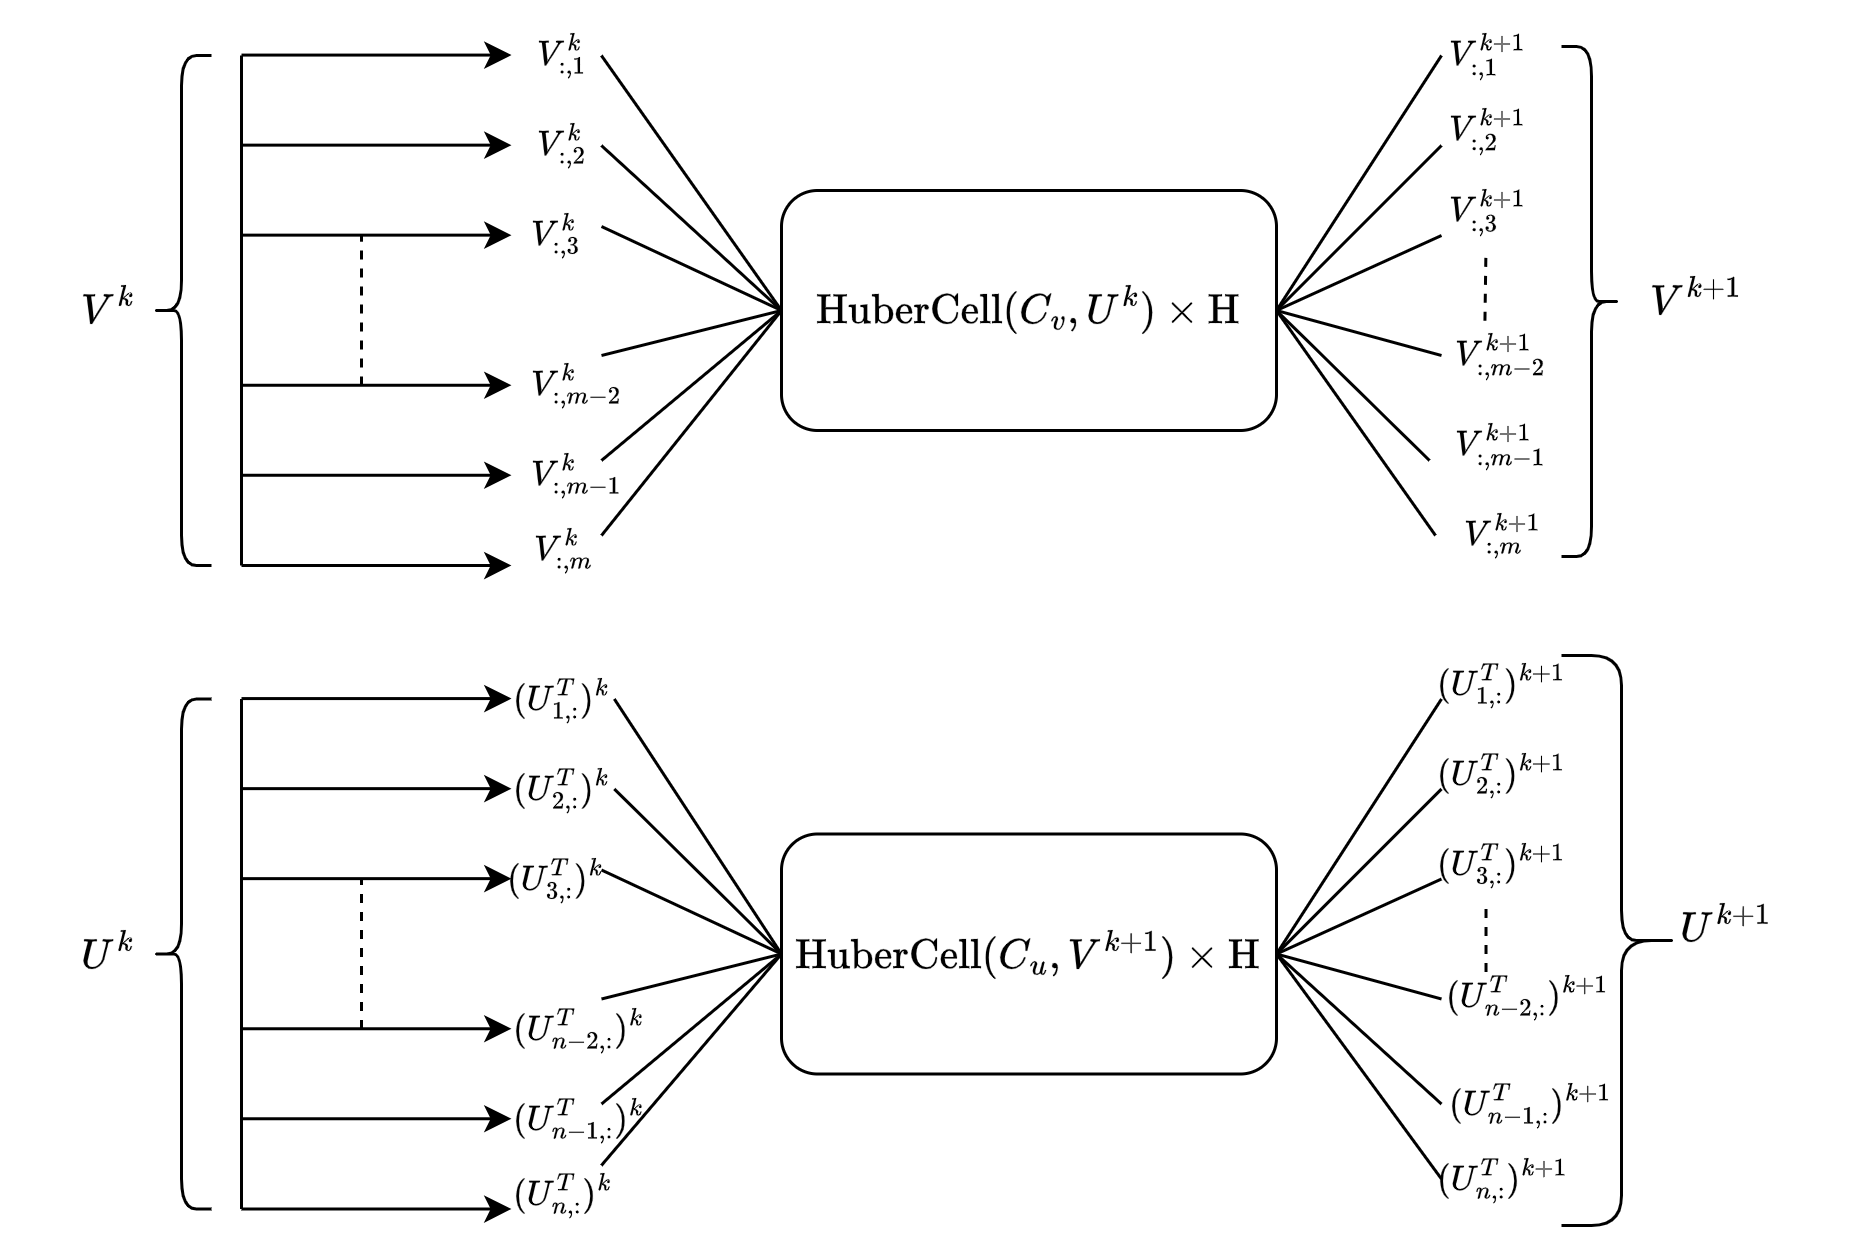
\includegraphics[width=\textwidth]{./Figures/huber-mc.png}
  \caption{ConvHuberMC-Net Architecture}
  \label{fig: arch1}
\end{figure}

We explain this architecture one by one. The neural network receives two inputs, $U$ and $V$ both initially randomly initialized from a standard normal. We then go ahead and sequentially update V followed by U. as shown in the above iterative version. Therefore by similarity, we consider the individuals columns of $V$, and rows of $U$. Each column of V and U go through a \textit{HuberCell} which is characterized by the exact Algorithm \ref{algo: 4} as discussed above. Note that each row/column update is accompanied by two arguments $C_i$ and current state of the other matrix. $C_i$ where $i \in {u, v}$ denotes the set of all learnable convolution maps (their hyperparameters such as stride etc discussed in section 4) for the matrix $U$ and $V$ respectively, all initialized to identity maps at the beginning for each update of row/column of $U$/$V$. Note that both matrix updates can be parallelized hence has much prospect in terms of computational ease. The convolution maps inclusion have been done in a very straightforward way by simply passing the convolution map to the corresponding $X^{+}$ for a specific update. This had two benefits. If we were to check the original paper of M-estimation being used to address RMC, the number of iterations $N_{iter}$ required for proper convergence was $500$. However, by making including these learnable parameters, we greatly reduce the number of iterations for a similar performance for some combinations as low as 2. This is precisely what $H$ denotes i.e. the $N_{iter}$ for a specific update. This is as simple as stacking HuberCells, one on top of another. In terms of computation ease, also note that the calculation of pseudoinverse only happens $H$ times compared to hundreds of times for the iterative version, again reducing the computational burden. 

After the HuberCell update, we get the updated column/row which are concatenated to form the updated U and V matrix. This update of U and V happens in same layer (\(k\)th layer as shown above). 

Now we go ahead and discuss briefly the state of the art methods \(\ell_0\)-BCD and \(\ell_p\)-reg.

\subsubsection{\(\ell_0\)-BCD Algorithm}

We will be going by the similar problem formulation as in \textbf{ALM} but this time we assume the sampled/incomplete matrix $D_{\Omega}$ has been exposed to impulsive Gaussian noise more specifically it can be decomposed as follows.

$$D_{\Omega} = \Tilde{D_{\Omega}} + G_{\Omega} + S_{\Omega}$$

where we consider the sampled and noisy matrix $D_{\Omega}$ can be decomposed into a noisy-free but sampled component $\Tilde{D_{\Omega}}$, Gaussian noise with small power/variance $G_{\Omega}$ and sparse impulsive Gaussian noises with high power, $S_{\Omega}$. We then formulate the \textit{robust} matrix completion (RMC) problem using matrix factorization and breaking the matrix of interest, $\Tilde{D_{\Omega}}$ into a product of two similar lower dimensional matrices, $U, V$.

\begin{equation}
\min_{U, V, S} \lVert D_{\Omega} - (UV)_{\Omega} - S_{\Omega} \rVert_F^{2} + \mu \lVert S_{\Omega} \rVert_0
\label{eq19}
\end{equation}
where $U \in \mathcal{R}^{M \times r}$ and $V \in \mathcal{R}^{r \times N}$
 and $r$ is the assumed rank of the original matrix $D$. 
Furthermore,  $S_0$ is utilized to separate outliers (sparse noise) from $D_{\Omega}$, and $\lVert D_{\Omega} - (UV)_{\Omega} - S_{\Omega} \rVert_F^{2}$ is able to resist the Gaussian noise, and $\mu > 0$ is the penalty parameter which controls the sparsity of $S$ and is automatically updated by a \textit{Laplacian} kernel-based method. \\ 

Using block coordinate descent (BCD) we are able to formulate this problem into further 3 sub-problems leading to the following iterative procedure: 

\begin{align}
U^{k+1} & = \arg \min_U \lVert D_{\Omega} - (UV^k)_{\Omega}  - S^{k}_{\Omega} \rVert_F^2 \\
V^{k+1} & = \arg \min_V \lVert D_{\Omega} - (U^{k+1}V)_{\Omega} - S^{k}_{\Omega} \rVert_F^2 \\
S^{k+1} & = \arg \min_S \lVert N^{k+1}_{\Omega} - S_{\Omega} \rVert + \mu^{k+1} \|S_{\Omega}\|_{0}
\end{align}

where $N^{k+1}_{\Omega} = D_{\Omega} - (U^{k+1}V^{k+1})_{\Omega}$. To solve (12) we use a hard-thresholding operator ${\tau}(\cdot)$ defined as follows: $$s^{k+1} = \tau_{\mu^{k+1}}(n^{k+1}) = \begin{cases}
(n^{k+1})_{i}, & \text{if} |(n^{k+1})_{i}| \geq \sqrt{\mu^{k+1}} \\
0, & \text{otherwise}
\end{cases}$$

We have used small letters $s$ and $n$ to denote their capital letter counterparts but with only non-zero entries. Mathematically, $s \in \mathcal{R}^{\|\Omega\|_{1}}$ and similarly $n \in \mathcal{R}^{\|\Omega\|_{1}}$. \\ Also note that after updating $U$ and $V$ we first update $\mu$ the adaptive penalty term before updating S. Without going into much detail how this is updated, the following algorithm summarizes the key steps in finding $\mu$ per iteration step. 

\begin{algorithm}
\caption{Outlier Detector Based on Laplacian Kernel}
\textbf{Input:} $n$ and $\epsilon$ \\
$\sigma^2 = 1.06 \times \min(\sigma_E, \frac{\text{IQR}}{1.34}) \times \text{dim}(n)^{-0.2}$ \\
$w = k_{\sigma}(n)$ \\
$\Psi = \{i\}$ based on $w_i \leq \epsilon$ \\
$\mu = \min(n^2_1, n^2_2, \ldots, n^2_i)$ s.t. $i \in \Psi$ \\
\textbf{Output:} $\mu$ and $\Psi$
\end{algorithm}

where $\sigma_E$ and $IQR$ are the standard deviation and interquartile range of $n$, respectively and $k_{\sigma}$ denotes the laplacian kernel defined as follows: \\
\[
k_{\sigma}(x - y) = \exp\left(-\frac{|x - y|}{\sigma}\right). 
\]
Note that $\sigma$ is called the kernel size or bandwidth. It is determined using the concept of kernel density estimation (\textit{Silverman's Rule} \cite{silverman}). The value of $k_{\sigma}(x - y)$ decreases as the value of $|x - y|$ increases. Especially, a very large value of $|x - y|$ results in $k_{\sigma}(x - y) = 0$. Hence, the Laplacian kernel has outlier detection capability. \\

After obtaining $\sigma$, we compute $w$ as $w = k_{\sigma}(n)$ where $w_i \leq \epsilon$ means that $n_i$ is an outlier. In our method, $\alpha$ is set to $10^{-20}$. Based on $w$, we obtain a coordinate set $\Psi$ of anomalies for $w_i \leq \epsilon$ and then $\mu$ is calculated as $\mu = \min(n^2_1, n^2_2, \ldots, n^2_i)$ s.t. $i \in \Psi$.

This algorithm is one of the top state of the art methods boasting its incredible low computational complexity and accuracy. The ingenious idea of theirs comes from their method of 'outlier detection' through the idea of updating 'adaptive penalty'. Also note that the update of S has a non-linear term of \(\ell_0\)-norm hence requires some sort of thresholding. However,$ \tau_{\mu^{k+1}}(n^{k+1})$ is nowhere near as computationally expensive as the SVT that we observed in ConvMC-Net.

Now that we have gone in much detail over our proposed models, ConvMC-Net and ConvHuberMC-Net as well as state of the art methods such $\ell_{0}$ - BCD, Huber's M-Estimation and $\ell_{p}$-reg, we are now fully equipped with the experimentation phase explained in detail in chapter 4.


\section{ Tools/Instruments}
\subsection{Simulation Software Packages}
We used the following sofware/libraries for our applications:
\begin{itemize}

\item Python
\item PyTorch
\item Numpy
\item MATLAB
\item Scipy

\end{itemize}
\subsection{Hardware Instruments}
We used computers provided by the Center for Urban Informatics, Technology, and Policy (CITY) at LUMS for training our deep learning based model. We used a custom built CPU with an Intel Core i7 processor and an NVIDIA 3090 GPU.